\documentclass[11pt]{article}
\usepackage{geometry}
\geometry{letterpaper}
\usepackage[parfill]{parskip} 
\usepackage{graphicx}
\usepackage{amssymb}

\title{CSCI503: Parallel Programming / Homework 1}
\author{Joe C. Student}

\begin{document}

\maketitle

\begin{enumerate}

\item[Q1.1] Sample answer to the homework written part.  Provided here for you as a sample report generated using {\LaTeX}.  As you can see from the sample graph shown in~\ref{fig:sample}, the performance is now what we had expected.  This is due to the fact that we did not run the code multiple times.

\begin{figure}[htbp]
   \centering
   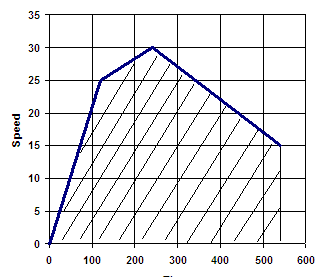
\includegraphics[width=2in]{example.png} 
   \caption{Performance comparison between serial and parallel code.}
   \label{fig:sample}
\end{figure}

\item[Q1.2] This is is another sample question.  Using the formular for speed up:

\begin{equation}
S_p = \frac{S_1}{S_n} 
\end{equation}


We can clearly see that $S_1$ must necessarily be bigger than $S_5$, otherwise we would not see any performance improvements.

\end{enumerate}

\end{document}
